% ============================================================
%  Anexo III - Estimación del tamaño y esfuerzo del proyecto
%  Sistema de Gestión Documental mediante Blockchain
%  Compilar con: lualatex AnexoIII_EstimacionPlanificacion.tex
% ============================================================

% ============================================================
% NOTA ENCODING (2026-03-27): Archivo corregido a UTF-8.
% Los caracteres acentuados (tildes) habian sido danados por
% una operacion de I/O con codificacion ISO-8859-1 en PS5.
% Patron 1 (AnexoI): U+FFFD para a/e/i/n/u; '?' para 'o'.
%   Solucion: diccionario de contexto + regex (fix_accents_v2.py, fix3.py).
% Patron 2 (AnexoII-V): todos los acentos como '?' literal.
%   Solucion: vacabulario de 462 entradas (fix_annexes_all.py, fix_final.py).
% REGLA: Siempre usar Python 3 + io.open(path,'w',encoding='utf-8').
%        NUNCA usar Set-Content de PowerShell 5 (anade BOM o rompe tildes).
% ============================================================
\documentclass[11pt, a4paper]{article}

\usepackage{fontspec}
\usepackage[spanish]{babel}
\usepackage{graphicx}
\usepackage{float}
\usepackage{amsmath}
\usepackage{amssymb}
\usepackage{xcolor}
\usepackage[protrusion=true,expansion=false]{microtype}
\usepackage{longtable}
\usepackage{array}
\usepackage{booktabs}
\usepackage{multirow}
\usepackage{enumitem}
\usepackage[
    colorlinks = true,
    linkcolor  = black,
    urlcolor   = black,
    citecolor  = black
]{hyperref}

\usepackage{geometry}
\geometry{
    left       = 2.5cm,
    right      = 2.5cm,
    top        = 3cm,
    bottom     = 2.5cm,
    headheight = 55pt,
    headsep    = 0.8cm
}

\usepackage{fancyhdr}
\pagestyle{fancy}
\fancyhf{}

\lhead{
\includegraphics[height=1.25cm]{USAL-Logo-3820702873.png}}
\rhead{\shortstack[r]{\fontsize{10}{12}\selectfont\textbf{\tituloInforme}\\[-1pt]\fontsize{10}{12}\selectfont\subtituloInforme}}

\renewcommand{\headrulewidth}{0pt}
\renewcommand{\footrulewidth}{0pt}

\cfoot{%
    \color{gray}\rule[0.5ex]{0.4\textwidth}{0.8pt}%
    \hspace{0.5cm}%
    \textcolor{black}{\textbf{\thepage}}%
    \hspace{0.5cm}%
    \color{gray}\rule[0.5ex]{0.4\textwidth}{0.8pt}%
}

\newcommand{\tituloInforme}{Anexo III: Estimación del tamaño y esfuerzo}
\newcommand{\subtituloInforme}{Sistema de Gestión Documental mediante Blockchain}
\newcommand{\asignatura}{Trabajo de Fin de Grado}
\newcommand{\autorUno}{David Pérez Velasco}
\newcommand{\tutorUno}{Gabriel Villarrubia González}
\newcommand{\tutorDos}{Sergio García González}

\graphicspath{{diagramas/}}
\begin{document}

\begin{titlepage}
    \centering
    \vspace*{1.5cm}

    {\scshape\LARGE Universidad de Salamanca \par}
    \vspace{1cm}
    {\scshape\Large Grado en Ingeniería Informática \par}
    \vspace{1.5cm}

    {\huge\bfseries \tituloInforme \par}
    \vspace{0.5cm}
    {\Large\bfseries \subtituloInforme \par}
    \vspace{1.8cm}

    
\includegraphics[width=0.34\textwidth]{USAL-Logo-3820702873.png}

    \vspace{1.8cm}

    {\Large\itshape \autorUno \par}
    \vspace{2cm}
    
    {\large Tutores: \par}
    \vspace{0.3cm}
    {\large \tutorUno \par}
    \vspace{0.2cm}
    {\large \tutorDos \par}

    \vfill

    \asignatura

    \vspace{1cm}
\end{titlepage}

\setcounter{page}{2}
\pagestyle{fancy}

\tableofcontents
\newpage

\listoffigures
\newpage

\listoftables
\newpage

\section{Introducción}

Este anexo presenta la estimación de esfuerzo y la planificación temporal del proyecto \textbf{DocumentChain}, un sistema de gestión documental basado en tecnología blockchain, utilizando la metodología del \textbf{Proceso Unificado (PU)} como marco de desarrollo iterativo e incremental, y la herramienta \textbf{EZEstimate} basada en \textbf{Puntos de Caso de Uso (UCP -- \textit{Use Case Points})} para la cuantificación del esfuerzo.

La estimación mediante UCP permite obtener una medida del tamaño funcional del sistema a partir de los actores y casos de uso identificados, ajustada a través de factores de complejidad técnica y del entorno. El Proceso Unificado organiza el desarrollo en cuatro fases principales (\textit{Inicio}, \textit{Elaboración}, \textit{Construcción} y \textit{Transición}), cada una dividida en iteraciones que permiten gestionar de forma progresiva la complejidad inherente a DocumentChain.

La complejidad particular de este proyecto reside en la integración de cuatro subsistemas heterogéneos: un \textit{backend} REST en Node.js, una base de datos relacional PostgreSQL, una capa de almacenamiento IPFS con proveedor configurable para la persistencia descentralizada y un \textit{smart contract} en Solidity desplegado sobre la red Ethereum. Esta arquitectura multi-capa justifica tanto la elección del Proceso Unificado como la necesidad de una estimación de esfuerzo rigurosa y justificada.

\section{Estudio de viabilidad del proyecto}

\subsection{Objetivos del sistema}

El desarrollo de DocumentChain sigue las cuatro fases fundamentales del Proceso Unificado, organizadas con dos iteraciones cada una, lo que permite abordar progresivamente la complejidad del sistema:

\begin{description}[leftmargin=2cm, style=nextline]
    \item[\textbf{Inicio}] Su objetivo es establecer el alcance del proyecto, identificar a los actores y sus interacciones principales, y evaluar la viabilidad del sistema. En la primera iteración se realiza un contacto inicial con el problema y el dominio; en la segunda se definen con precisión los objetivos, actores y casos de uso más relevantes, y se elabora la planificación inicial.

    \item[\textbf{Elaboración}] Su objetivo es estabilizar la arquitectura del sistema, completar el análisis de requisitos y reducir los riesgos técnicos. En la primera iteración se especifican en detalle los requisitos (IRQ, NFR) y se diseña la arquitectura general; en la segunda se diseñan los componentes más complejos (smart contract, cifrado híbrido de documentos y protección de claves) y se elaboran los diagramas UML y la documentación técnica.

    \item[\textbf{Construcción}] Su objetivo es implementar el sistema completo de forma iterativa. La primera iteración abarca los subsistemas centrales: autenticación, documentos, versionado, firmas, compartición y el frontend básico. La segunda iteración añade funcionalidades avanzadas: estadísticas, auditoría, administración, notificaciones y ajustes de rendimiento y seguridad.

    \item[\textbf{Transición}] Su objetivo es desplegar el sistema en el entorno de producción, validarlo con usuarios reales y cerrar el proyecto. La primera iteración contempla el despliegue completo y las pruebas finales; la segunda el cierre de la documentación académica y la entrega del TFG.
\end{description}

\subsection{Factores de complejidad técnica y del entorno}

\subsubsection{Factores de complejidad técnica}

El método UCP define 13 factores técnicos (T1--T13) que impactan la complejidad del proyecto. Cada factor se puntúa de 0 (sin impacto) a 5 (máximo impacto) y se multiplica por su peso predefinido para obtener el subtotal.

\begin{longtable}{|p{0.8cm}|p{7.5cm}|p{1.3cm}|p{1.8cm}|p{2cm}|}
\hline
\textbf{ID} & \textbf{Factor} & \textbf{Peso} & \textbf{Valoración} & \textbf{Subtotal} \\
\hline
\endfirsthead
\hline
\textbf{ID} & \textbf{Factor} & \textbf{Peso} & \textbf{Valoración} & \textbf{Subtotal} \\
\hline
\endhead
T1 & Sistema distribuido (Blockchain + IPFS + REST API) & 2.0 & 5 & 10.0 \\
\hline
T2 & Objetivos de rendimiento y tiempos de respuesta & 1.0 & 4 & 4.0 \\
\hline
T3 & Eficiencia del usuario final (UX intuitiva) & 1.0 & 4 & 4.0 \\
\hline
T4 & Procesamiento interno complejo (cifrado híbrido, blockchain) & 1.0 & 5 & 5.0 \\
\hline
T5 & Código reutilizable y modular & 1.0 & 4 & 4.0 \\
\hline
T6 & Facilidad de instalación (Docker Compose) & 0.5 & 3 & 1.5 \\
\hline
T7 & Facilidad de uso (interfaz web intuitiva) & 0.5 & 4 & 2.0 \\
\hline
T8 & Portabilidad (multi-plataforma vía navegador web) & 2.0 & 4 & 8.0 \\
\hline
T9 & Facilidad de cambio y mantenimiento & 1.0 & 4 & 4.0 \\
\hline
T10 & Concurrencia (múltiples usuarios simultáneos) & 1.0 & 4 & 4.0 \\
\hline
T11 & Seguridad especial (cifrado de documentos, control de acceso e inmutabilidad blockchain) & 1.0 & 5 & 5.0 \\
\hline
T12 & Acceso de terceros (wallets compatibles, nodos IPFS, Ethereum) & 1.0 & 5 & 5.0 \\
\hline
T13 & Facilidades de formación para usuarios & 1.0 & 3 & 3.0 \\
\hline
\multicolumn{4}{|r|}{\textbf{Total Factor Técnico (TF):}} & \textbf{59.5} \\
\hline
\caption{Factores de complejidad técnica (T1--T13)}
\end{longtable}

\vspace{0.5em}
\noindent El \textbf{Factor de Complejidad Técnica (TCF)} se calcula como:

\begin{equation}
\text{TCF} = 0{,}6 + (0{,}01 \times \text{TF}) = 0{,}6 + (0{,}01 \times 59{,}5) = \mathbf{1{,}195}
\end{equation}

Un TCF superior a 1,0 indica complejidad técnica elevada, consecuencia directa de la integración de blockchain, criptografía avanzada y almacenamiento distribuido.

\subsubsection{Factores del entorno}

El método UCP define 8 factores del entorno (E1--E8) relacionados con el equipo y el contexto de desarrollo. Los factores E7 y E8 tienen peso negativo, penalizando escenarios desfavorables.

\begin{longtable}{|p{0.8cm}|p{7.5cm}|p{1.3cm}|p{1.8cm}|p{2cm}|}
\hline
\textbf{ID} & \textbf{Factor} & \textbf{Peso} & \textbf{Valoración} & \textbf{Subtotal} \\
\hline
\endfirsthead
\hline
\textbf{ID} & \textbf{Factor} & \textbf{Peso} & \textbf{Valoración} & \textbf{Subtotal} \\
\hline
\endhead
E1 & Familiaridad con el modelo de proyecto (TFG académico) & 1.5 & 3 & 4.5 \\
\hline
E2 & Experiencia en la aplicación (blockchain, nuevo dominio) & 0.5 & 2 & 1.0 \\
\hline
E3 & Experiencia en orientación a objetos (TypeScript) & 1.0 & 4 & 4.0 \\
\hline
E4 & Capacidad del analista líder (autónomo, tutorizado) & 0.5 & 3 & 1.5 \\
\hline
E5 & Motivación del equipo (alta --- proyecto TFG personal) & 1.0 & 5 & 5.0 \\
\hline
E6 & Estabilidad de requisitos (bien definidos, pocos cambios) & 2.0 & 4 & 8.0 \\
\hline
E7 & Personal a tiempo parcial (estudiante, 6h/día) & -1.0 & 3 & -3.0 \\
\hline
E8 & Dificultad del lenguaje (TypeScript + Solidity) & -1.0 & 3 & -3.0 \\
\hline
\multicolumn{4}{|r|}{\textbf{Total Factor Ambiental (EF):}} & \textbf{18.0} \\
\hline
\caption{Factores del entorno (E1--E8)}
\end{longtable}

\vspace{0.5em}
\noindent El \textbf{Factor de Complejidad del Entorno (ECF)} se calcula como:

\begin{equation}
\text{ECF} = 1{,}4 + (-0{,}03 \times \text{EF}) = 1{,}4 + (-0{,}03 \times 18{,}0) = \mathbf{0{,}86}
\end{equation}

Un ECF inferior a 1,0 refleja factores negativos como la curva de aprendizaje en blockchain y la dedicación a tiempo parcial, que reducen ligeramente la productividad estimada.

\subsection{Lista de casos de uso y representación de actores}

El sistema DocumentChain cuenta con \textbf{5 actores} y \textbf{42 casos de uso} distribuidos en 9 paquetes funcionales. Para facilitar la lectura, los diagramas de actores se presentan agrupados por paquete de gestión.

\begin{figure}[H]
    \centering
    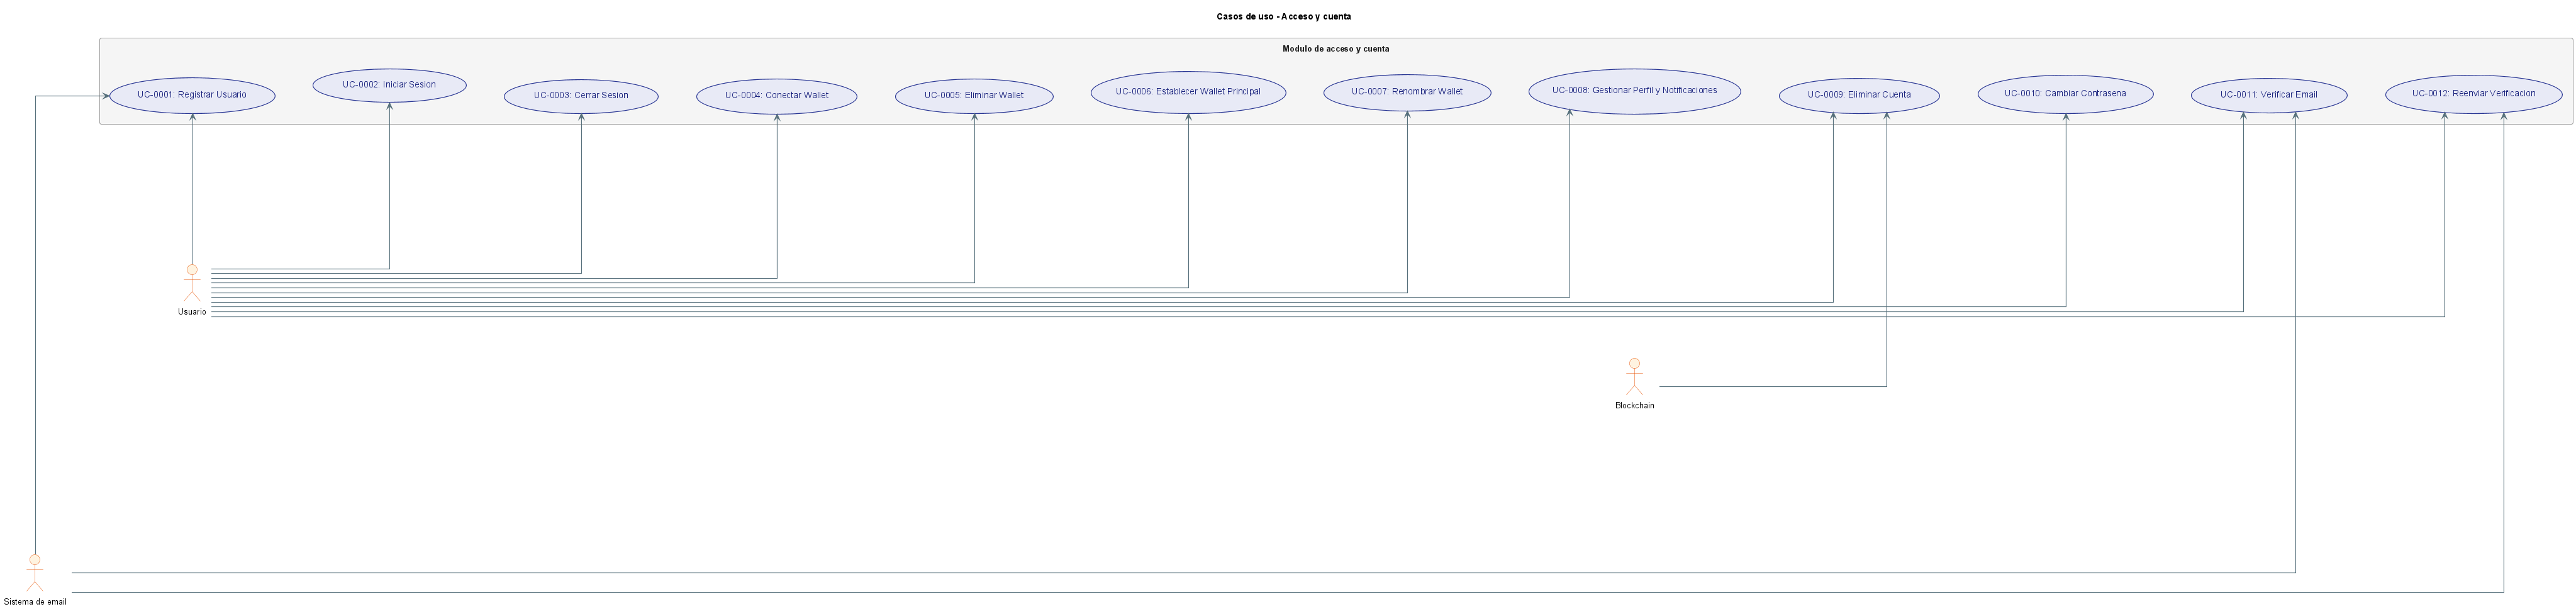
\includegraphics[width=0.75\linewidth]{diagramas/uc_acceso.png}
    \caption{Diagrama de casos de uso: Paquete de Gestión de Acceso}
    \label{fig:uc_acceso}
\end{figure}

\begin{figure}[H]
    \centering
    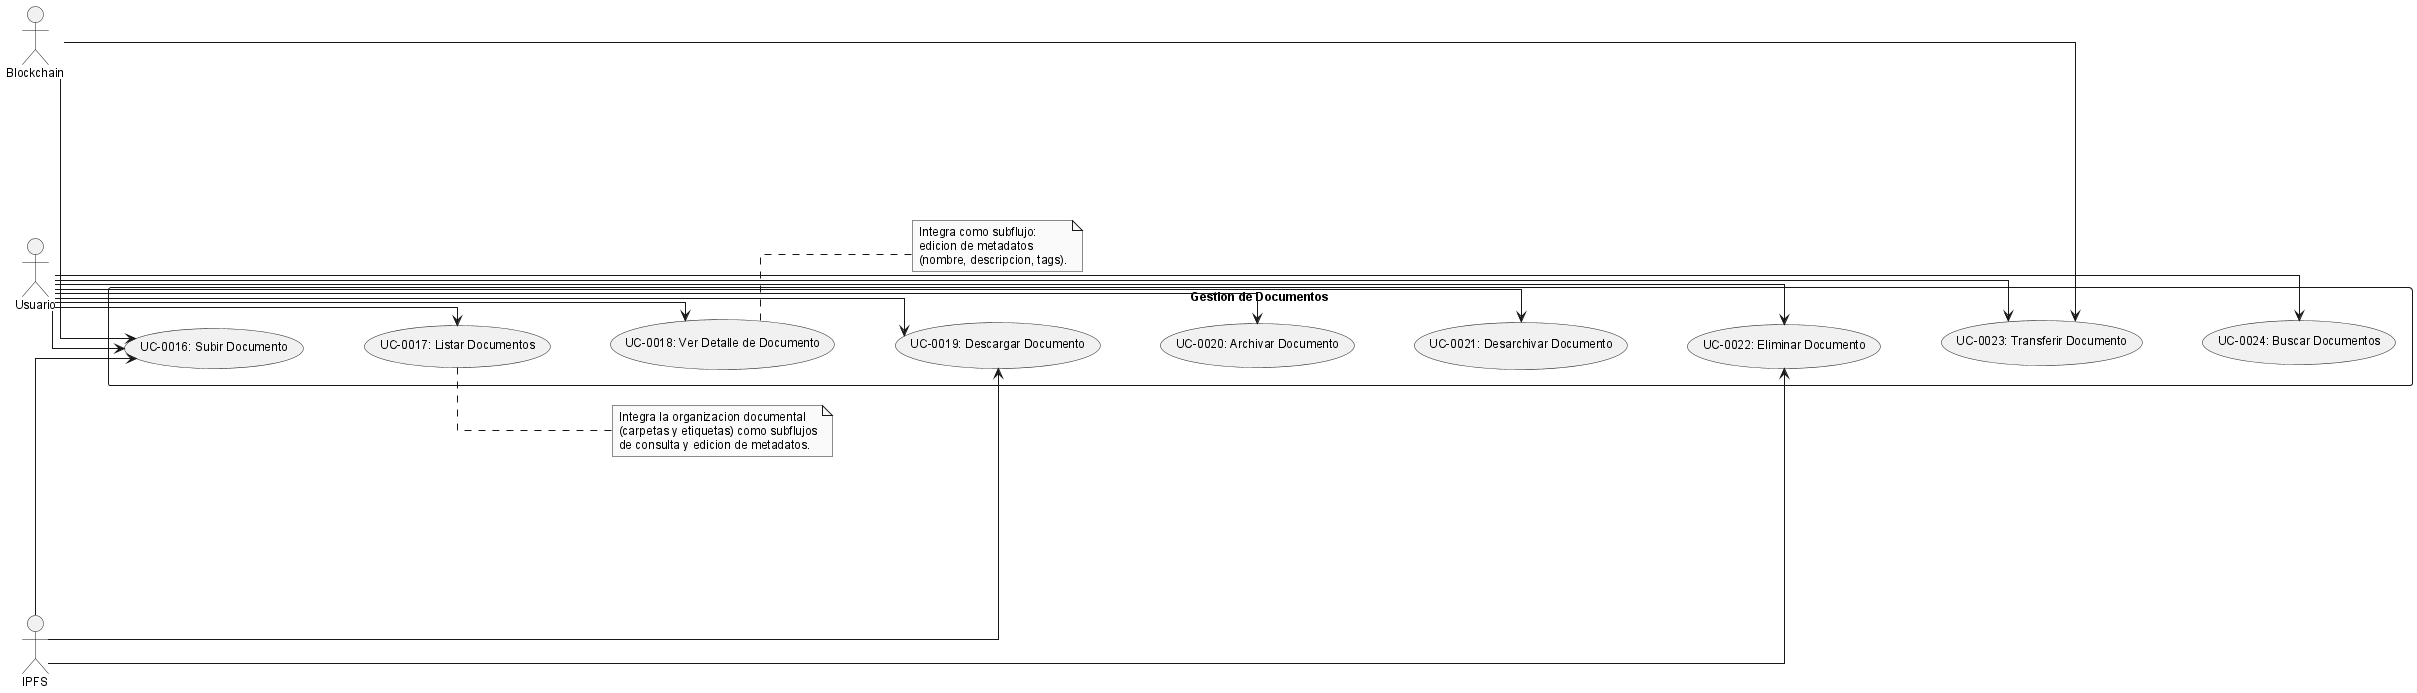
\includegraphics[width=0.80\linewidth]{diagramas/uc_documentos.png}
    \caption{Diagrama de casos de uso: Paquete de Gestión de Documentos}
    \label{fig:uc_documentos}
\end{figure}

\begin{figure}[H]
    \centering
    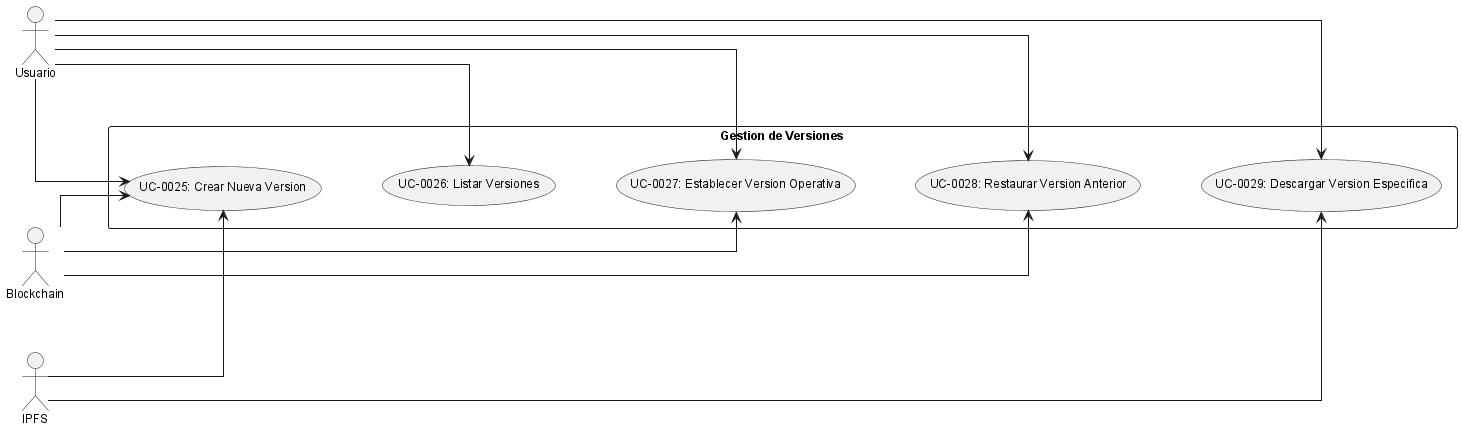
\includegraphics[width=0.72\linewidth]{diagramas/uc_versiones.png}
    \caption{Diagrama de casos de uso: Paquete de Gestión de Versiones}
    \label{fig:uc_versiones}
\end{figure}

\begin{figure}[H]
    \centering
    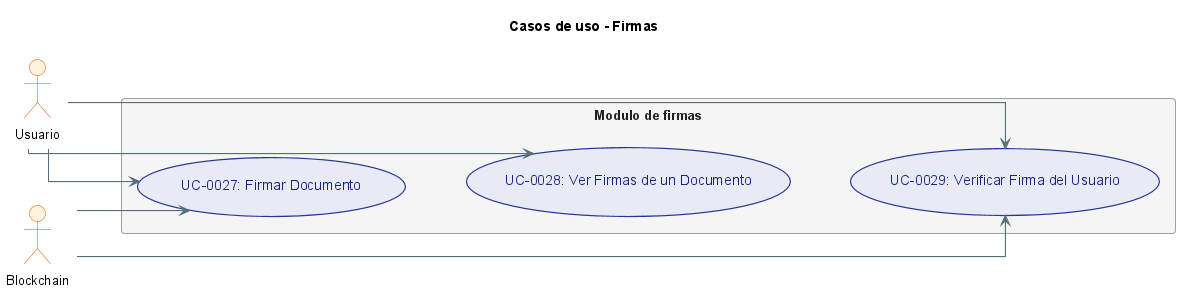
\includegraphics[width=0.60\linewidth]{diagramas/uc_firmas.png}
    \caption{Diagrama de casos de uso: Paquete de Gestión de Firmas}
    \label{fig:uc_firmas}
\end{figure}

\begin{figure}[H]
    \centering
    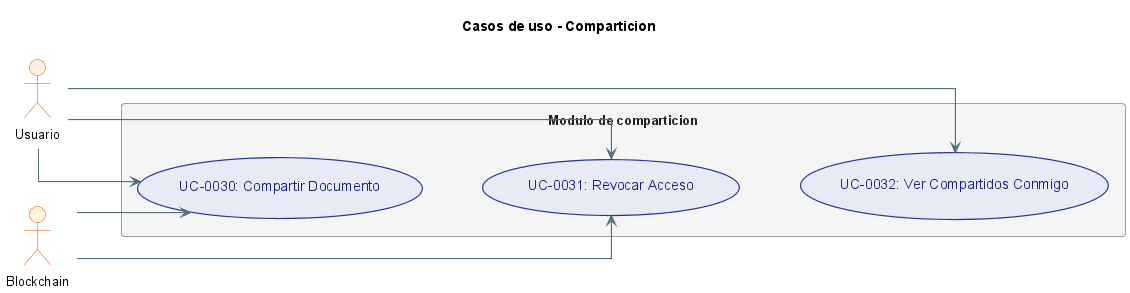
\includegraphics[width=0.68\linewidth]{diagramas/uc_comparticion.png}
    \caption{Diagrama de casos de uso: Paquete de Gestión de Compartición}
    \label{fig:uc_comparticion}
\end{figure}

\begin{figure}[H]
    \centering
    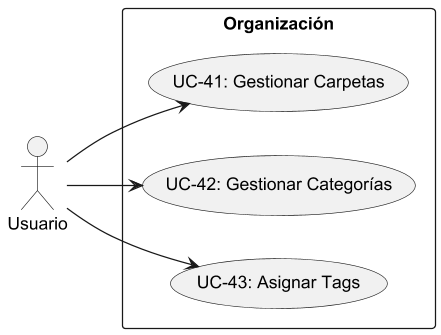
\includegraphics[width=0.55\linewidth]{diagramas/uc_organizacion.png}
    \caption{Diagrama de casos de uso: Paquete de Organización}
    \label{fig:uc_organizacion}
\end{figure}

\begin{figure}[H]
    \centering
    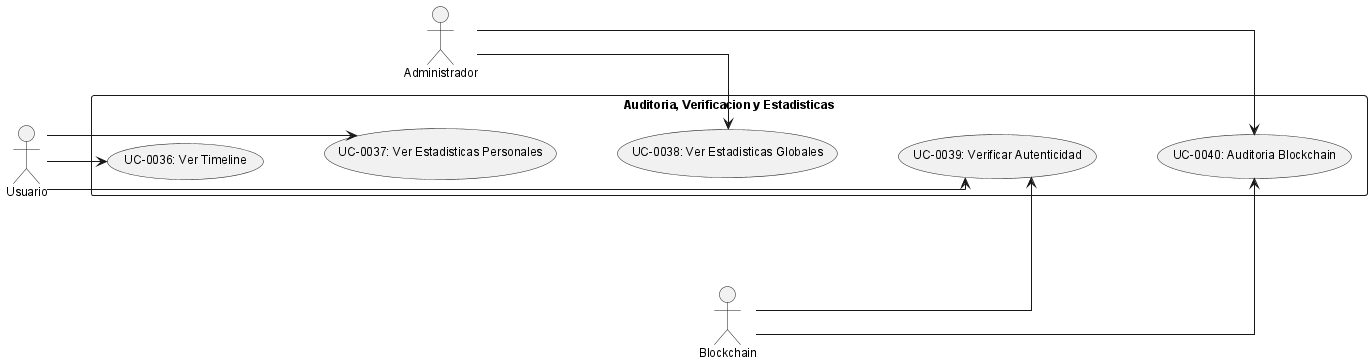
\includegraphics[width=0.72\linewidth]{diagramas/uc_auditoria.png}
    \caption{Diagrama de casos de uso: Paquete de Auditoría y Estadísticas}
    \label{fig:uc_auditoria}
\end{figure}

\begin{figure}[H]
    \centering
    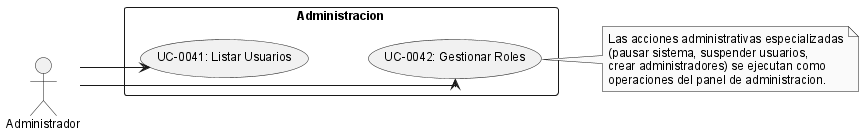
\includegraphics[width=0.68\linewidth]{diagramas/uc_administracion.png}
    \caption{Diagrama de casos de uso: Paquete de Administración}
    \label{fig:uc_administracion}
\end{figure}

\begin{figure}[H]
    \centering
    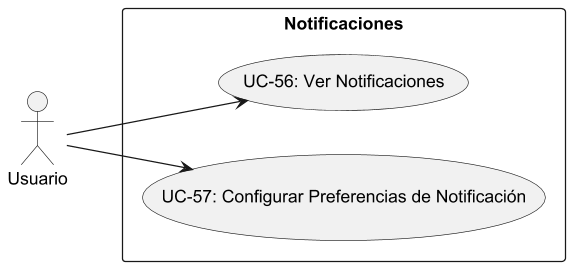
\includegraphics[width=0.55\linewidth]{diagramas/uc_notificaciones.png}
    \caption{Diagrama de casos de uso: Paquete de Notificaciones}
    \label{fig:uc_notificaciones}
\end{figure}

\subsection{Actores del sistema}

Los actores del sistema se clasifican según su complejidad de interacción:

\begin{itemize}
    \item \textbf{Simple} (peso 1): Sistema externo con API definida
    \item \textbf{Medio} (peso 2): Sistema con protocolo o interfaz textual
    \item \textbf{Complejo} (peso 3): Usuario a través de interfaz gráfica
\end{itemize}

\begin{table}[H]
\centering
\begin{tabular}{|l|p{7cm}|l|c|}
\hline
\textbf{ID} & \textbf{Actor} & \textbf{Tipo} & \textbf{Peso} \\
\hline
ACT-01 & Usuario registrado (interfaz web compleja) & Complejo & 3 \\
\hline
ACT-02 & Administrador (interfaz web de administración) & Complejo & 3 \\
\hline
ACT-03 & Smart Contract DocumentRegistry (API JSON-RPC) & Simple & 1 \\
\hline
ACT-04 & Proveedor IPFS (API HTTP) & Simple & 1 \\
\hline
ACT-05 & Sistema de Email SMTP & Medio & 2 \\
\hline
\multicolumn{3}{|r|}{\textbf{Total Peso de Actores (UAW):}} & \textbf{10} \\
\hline
\end{tabular}
\caption{Clasificación de actores del sistema}
\end{table}

\begin{figure}[H]
    \centering
    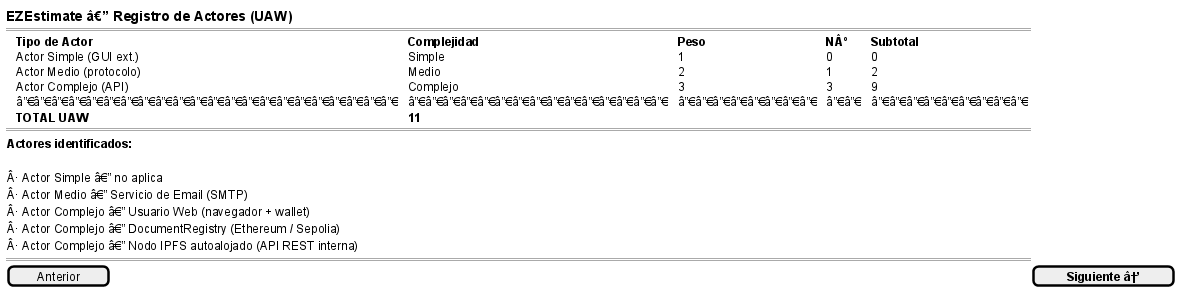
\includegraphics[width=0.88\linewidth]{ezestimate-actors.png}
    \caption{EZEstimate --- Pantalla de registro y ponderación de actores (UAW)}
    \label{fig:ezestimate-actors}
\end{figure}

\subsection{Casos de uso}

Los casos de uso se clasifican según el número de transacciones (interacciones) necesarias para completarlos:

\begin{itemize}
    \item \textbf{Simple} (1--3 transacciones, peso 5)
    \item \textbf{Medio} (4--7 transacciones, peso 10)
    \item \textbf{Complejo} (8 o más transacciones, peso 15)
\end{itemize}

\subsubsection*{Paquete: Gestión de Acceso}

\begin{longtable}{|p{1.8cm}|p{6.5cm}|p{3cm}|p{1.5cm}|}
\hline
\textbf{ID} & \textbf{Caso de Uso} & \textbf{Complejidad (Tx)} & \textbf{Peso} \\
\hline
\endfirsthead
\hline
\textbf{ID} & \textbf{Caso de Uso} & \textbf{Complejidad (Tx)} & \textbf{Peso} \\
\hline
\endhead
UC-0001 & Registrar Usuario & Complejo (10) & 15 \\
\hline
UC-0003 & Iniciar Sesión con Credenciales & Medio (6) & 10 \\
\hline
UC-0005 & Iniciar Sesión con Wallet & Medio (5) & 10 \\
\hline
UC-0006 & Cerrar Sesión & Simple (2) & 5 \\
\hline
UC-0010 & Ver Perfil & Simple (2) & 5 \\
\hline
UC-0013 & Editar Perfil & Medio (5) & 10 \\
\hline
UC-0014 & Conectar Wallet Adicional & Medio (6) & 10 \\
\hline
UC-0015 & Desconectar Wallet & Simple (2) & 5 \\
\hline
UC-0017 & Recuperar Contraseña & Medio (7) & 10 \\
\hline
\multicolumn{3}{|r|}{\textbf{Subtotal Gestión de Acceso:}} & \textbf{80} \\
\hline
\caption{Casos de uso --- Gestión de Acceso}
\end{longtable}

\subsubsection*{Paquete: Gestión de Documentos}

\begin{longtable}{|p{1.8cm}|p{6.5cm}|p{3cm}|p{1.5cm}|}
\hline
\textbf{ID} & \textbf{Caso de Uso} & \textbf{Complejidad (Tx)} & \textbf{Peso} \\
\hline
\endfirsthead
\hline
\textbf{ID} & \textbf{Caso de Uso} & \textbf{Complejidad (Tx)} & \textbf{Peso} \\
\hline
\endhead
UC-0019 & Subir Documento & Complejo (12) & 15 \\
\hline
UC-0020 & Listar Documentos & Medio (5) & 10 \\
\hline
UC-0021 & Ver Detalles de Documento & Medio (4) & 10 \\
\hline
UC-0022 & Descargar Documento & Complejo (9) & 15 \\
\hline
UC-0023 & Archivar Documento & Medio (5) & 10 \\
\hline
UC-0025 & Eliminar Documento & Medio (5) & 10 \\
\hline
UC-0026 & Editar Metadatos de Documento & Simple (3) & 5 \\
\hline
UC-0028 & Buscar Documentos & Complejo (8) & 15 \\
\hline
\multicolumn{3}{|r|}{\textbf{Subtotal Gestión de Documentos:}} & \textbf{90} \\
\hline
\caption{Casos de uso --- Gestión de Documentos}
\end{longtable}

\subsubsection*{Paquete: Gestión de Versiones}

\begin{longtable}{|p{1.8cm}|p{6.5cm}|p{3cm}|p{1.5cm}|}
\hline
\textbf{ID} & \textbf{Caso de Uso} & \textbf{Complejidad (Tx)} & \textbf{Peso} \\
\hline
\endfirsthead
\hline
\textbf{ID} & \textbf{Caso de Uso} & \textbf{Complejidad (Tx)} & \textbf{Peso} \\
\hline
\endhead
UC-0029 & Crear Nueva Versión & Complejo (10) & 15 \\
\hline
UC-0030 & Listar Versiones & Simple (2) & 5 \\
\hline
UC-0031 & Establecer Versión Operativa & Simple (2) & 5 \\
\hline
UC-0032 & Restaurar Versión Anterior & Medio (7) & 10 \\
\hline
UC-0033 & Descargar Versión Específica & Medio (5) & 10 \\
\hline
\multicolumn{3}{|r|}{\textbf{Subtotal Gestión de Versiones:}} & \textbf{45} \\
\hline
\caption{Casos de uso --- Gestión de Versiones}
\end{longtable}

\subsubsection*{Paquete: Gestión de Firmas}

\begin{longtable}{|p{1.8cm}|p{6.5cm}|p{3cm}|p{1.5cm}|}
\hline
\textbf{ID} & \textbf{Caso de Uso} & \textbf{Complejidad (Tx)} & \textbf{Peso} \\
\hline
\endfirsthead
\hline
\textbf{ID} & \textbf{Caso de Uso} & \textbf{Complejidad (Tx)} & \textbf{Peso} \\
\hline
\endhead
UC-0034 & Firmar Documento & Complejo (11) & 15 \\
\hline
UC-0035 & Listar Firmas & Simple (2) & 5 \\
\hline
UC-0036 & Verificar Firma & Medio (6) & 10 \\
\hline
\multicolumn{3}{|r|}{\textbf{Subtotal Gestión de Firmas:}} & \textbf{30} \\
\hline
\caption{Casos de uso --- Gestión de Firmas}
\end{longtable}

\subsubsection*{Paquete: Gestión de Compartición}

\begin{longtable}{|p{1.8cm}|p{6.5cm}|p{3cm}|p{1.5cm}|}
\hline
\textbf{ID} & \textbf{Caso de Uso} & \textbf{Complejidad (Tx)} & \textbf{Peso} \\
\hline
\endfirsthead
\hline
\textbf{ID} & \textbf{Caso de Uso} & \textbf{Complejidad (Tx)} & \textbf{Peso} \\
\hline
\endhead
UC-0037 & Compartir Documento & Complejo (10) & 15 \\
\hline
UC-0038 & Modificar Permisos & Medio (6) & 10 \\
\hline
UC-0039 & Revocar Acceso & Medio (5) & 10 \\
\hline
UC-0040 & Transferir Propiedad & Complejo (9) & 15 \\
\hline
\multicolumn{3}{|r|}{\textbf{Subtotal Gestión de Compartición:}} & \textbf{50} \\
\hline
\caption{Casos de uso --- Gestión de Compartición}
\end{longtable}

\subsubsection*{Paquete: Organización}

\begin{longtable}{|p{1.8cm}|p{6.5cm}|p{3cm}|p{1.5cm}|}
\hline
\textbf{ID} & \textbf{Caso de Uso} & \textbf{Complejidad (Tx)} & \textbf{Peso} \\
\hline
\endfirsthead
\hline
\textbf{ID} & \textbf{Caso de Uso} & \textbf{Complejidad (Tx)} & \textbf{Peso} \\
\hline
\endhead
UC-0041 & Gestionar Carpetas & Medio (6) & 10 \\
\hline
UC-0042 & Gestionar Categorías & Medio (6) & 10 \\
\hline
UC-0043 & Asignar Tags & Simple (3) & 5 \\
\hline
\multicolumn{3}{|r|}{\textbf{Subtotal Organización:}} & \textbf{25} \\
\hline
\caption{Casos de uso --- Organización}
\end{longtable}

\subsubsection*{Paquete: Auditoría y Estadísticas}

\begin{longtable}{|p{1.8cm}|p{6.5cm}|p{3cm}|p{1.5cm}|}
\hline
\textbf{ID} & \textbf{Caso de Uso} & \textbf{Complejidad (Tx)} & \textbf{Peso} \\
\hline
\endfirsthead
\hline
\textbf{ID} & \textbf{Caso de Uso} & \textbf{Complejidad (Tx)} & \textbf{Peso} \\
\hline
\endhead
UC-0044 & Ver Timeline de Eventos & Medio (5) & 10 \\
\hline
UC-0045 & Ver Estadísticas Personales & Medio (5) & 10 \\
\hline
UC-0046 & Auditar Documento en Blockchain & Medio (6) & 10 \\
\hline
UC-0048 & Exportar Reporte de Actividad & Medio (5) & 10 \\
\hline
\multicolumn{3}{|r|}{\textbf{Subtotal Auditoría y Estadísticas:}} & \textbf{40} \\
\hline
\caption{Casos de uso --- Auditoría y Estadísticas}
\end{longtable}

\subsubsection*{Paquete: Administración}

\begin{longtable}{|p{1.8cm}|p{6.5cm}|p{3cm}|p{1.5cm}|}
\hline
\textbf{ID} & \textbf{Caso de Uso} & \textbf{Complejidad (Tx)} & \textbf{Peso} \\
\hline
\endfirsthead
\hline
\textbf{ID} & \textbf{Caso de Uso} & \textbf{Complejidad (Tx)} & \textbf{Peso} \\
\hline
\endhead
UC-0049 & Gestionar Usuarios (Admin) & Complejo (10) & 15 \\
\hline
UC-0050 & Ver Estadísticas del Sistema & Medio (5) & 10 \\
\hline
UC-0052 & Pausar Sistema (Circuit Breaker) & Medio (6) & 10 \\
\hline
UC-0054 & Auditar Blockchain (Admin) & Medio (6) & 10 \\
\hline
\multicolumn{3}{|r|}{\textbf{Subtotal Administración:}} & \textbf{45} \\
\hline
\caption{Casos de uso --- Administración}
\end{longtable}

\subsubsection*{Paquete: Notificaciones}

\begin{longtable}{|p{1.8cm}|p{6.5cm}|p{3cm}|p{1.5cm}|}
\hline
\textbf{ID} & \textbf{Caso de Uso} & \textbf{Complejidad (Tx)} & \textbf{Peso} \\
\hline
\endfirsthead
\hline
\textbf{ID} & \textbf{Caso de Uso} & \textbf{Complejidad (Tx)} & \textbf{Peso} \\
\hline
\endhead
UC-0056 & Ver Notificaciones & Simple (2) & 5 \\
\hline
UC-0057 & Configurar Preferencias de Notificación & Medio (4) & 10 \\
\hline
\multicolumn{3}{|r|}{\textbf{Subtotal Notificaciones:}} & \textbf{15} \\
\hline
\caption{Casos de uso --- Notificaciones}
\end{longtable}

\subsubsection*{Resumen de clasificación}

\begin{table}[H]
\centering
\begin{tabular}{|l|c|c|c|}
\hline
\textbf{Complejidad} & \textbf{Cantidad} & \textbf{Peso unitario} & \textbf{Total} \\
\hline
Simple (1--3 Tx) & 9 & 5 & 45 \\
\hline
Medio (4--7 Tx) & 24 & 10 & 240 \\
\hline
Complejo (8+ Tx) & 9 & 15 & 135 \\
\hline
\textbf{Total} & \textbf{42} & --- & \textbf{420} \\
\hline
\end{tabular}
\caption{Resumen de Pesos de Casos de Uso (UUCW)}
\end{table}

\begin{figure}[H]
    \centering
    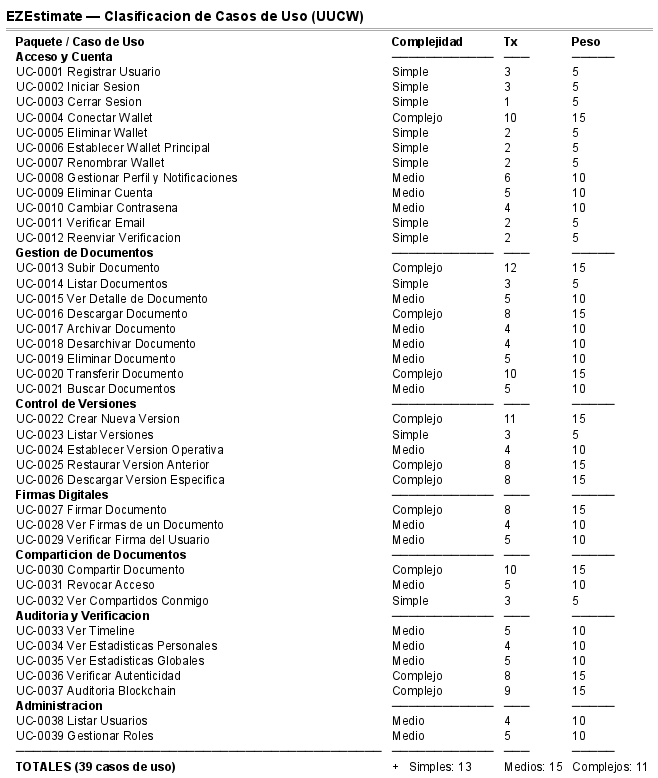
\includegraphics[width=0.92\linewidth]{ezestimate-uc-1.png}
    \caption{EZEstimate --- Pantalla de clasificación de casos de uso por complejidad (UUCW)}
    \label{fig:ezestimate-uc}
\end{figure}

\subsection{Conclusión y análisis de resultados}

A partir de los factores y clasificaciones anteriores, se aplica la metodología UCP para obtener los Puntos de Caso de Uso Ajustados (\textit{UCP}):

\begin{align}
\text{UUCP} &= \text{UAW} + \text{UUCW} = 10 + 420 = \mathbf{430} \\[4pt]
\text{UCP} &= \text{UUCP} \times \text{TCF} \times \text{ECF} = 430 \times 1{,}195 \times 0{,}86 \approx \mathbf{442}
\end{align}

Estos valores han sido introducidos en la herramienta \textbf{EZEstimate}, que proporciona una estimación del esfuerzo total considerando los factores de complejidad técnica y del entorno. El resultado obtenido se muestra en la siguiente ilustración:

\begin{figure}[H]
    \centering
    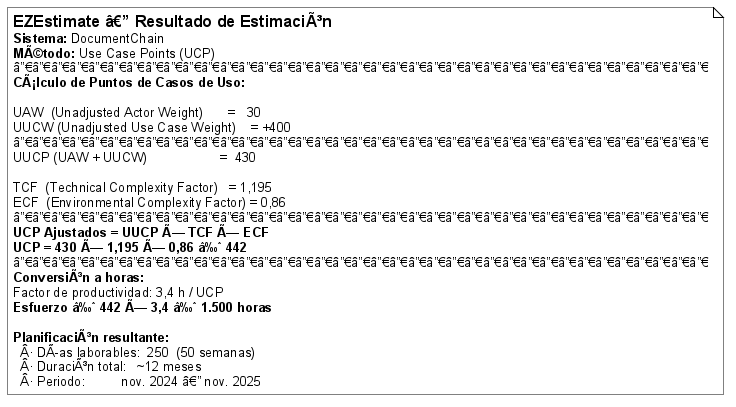
\includegraphics[width=0.92\linewidth]{ezestimate.png}
    \caption{EZEstimate --- Factores TCF y ECF con resultado final de la estimación UCP}
    \label{fig:ezestimate}
\end{figure}

\begin{table}[H]
\centering
\begin{tabular}{|l|r|}
\hline
\textbf{Parámetro} & \textbf{Valor} \\
\hline
Puntos de Caso de Uso Sin Ajustar (UUCP) & 430 \\
\hline
Factor de Complejidad Técnica (TCF) & 1{,}195 \\
\hline
Factor del Entorno (ECF) & 0{,}86 \\
\hline
Puntos de Caso de Uso Ajustados (UCP) & 442 \\
\hline
Estimación de esfuerzo total & 1.500 horas \\
\hline
Horas totales estimadas & 1.500 horas \\
\hline
Dedicación real & $\sim$10 h/día (incluye fines de semana) \\
\hline
Duración efectiva & 6 meses \\
\hline
Período de ejecución & 1 dic.\ 2025 -- 15 may.\ 2026 \\
\hline
\end{tabular}
\caption{Resumen de la estimación de esfuerzo mediante EZEstimate}
\end{table}

El cómputo de 1.500 horas de trabajo efectivo se ha obtenido aplicando un factor de productividad de \textbf{3,4 h/UCP}, recogido por la herramienta EZEstimate como valor de referencia para proyectos académicos con un único desarrollador y tecnologías parcialmente novedosas. El resultado teórico de la herramienta representa el esfuerzo bruto del proyecto. En la práctica, este esfuerzo se ha materializado en un período de \textbf{aproximadamente seis meses de trabajo intensivo} (del 1 de diciembre de 2025 a mediados de mayo de 2026), con una dedicación media de \textbf{10 horas diarias} que incluye fines de semana y adaptada a los compromisos académicos concurrentes, lo que equivale en cómputo global a las 1.500 horas estimadas.

\section{Planificación temporal}

\subsection{Descripción de tareas, subtareas e hitos}

A continuación se presenta la relación completa de tareas, subtareas e hitos del proyecto DocumentChain, organizada según las fases del Proceso Unificado. Los hitos aparecen en negrita y están identificados por el símbolo $\blacklozenge$.

\begin{longtable}{|p{1cm}|p{5.5cm}|p{1.5cm}|p{5.5cm}|}
\hline
\textbf{Núm.} & \textbf{Tarea o hito} & \textbf{Prec.} & \textbf{Descripción} \\
\hline
\endfirsthead
\hline
\textbf{Núm.} & \textbf{Tarea o hito} & \textbf{Prec.} & \textbf{Descripción} \\
\hline
\endhead
\multicolumn{4}{|c|}{\textit{\textbf{--- FASE: INICIO --- Iteración 1 ---}}} \\
\hline
1 & Reunión inicial con tutores & --- & Primera toma de contacto con el proyecto. Definición del tema, alcance general y tutores asignados. \\
\hline
2 & Análisis del dominio del problema & 1 & Estudio del campo de la gestión documental y del estado del arte blockchain aplicado a documentos. \\
\hline
3 & Estudio de soluciones existentes & 2 & Revisión de sistemas similares (Google Drive, Docusign) y sus carencias respecto a privacidad y trazabilidad. \\
\hline
4 & \textbf{$\blacklozenge$ Fin Iteración 1 (Inicio)} & 3 & Hito que marca el final de la primera iteración de la fase de Inicio. \\
\hline
\multicolumn{4}{|c|}{\textit{\textbf{--- FASE: INICIO --- Iteración 2 ---}}} \\
\hline
5 & Definición del alcance y objetivos & 4 & Especificación de los objetivos del sistema (OBJ-0001 a OBJ-0006) y sus restricciones. \\
\hline
6 & Identificación de actores y UC iniciales & 5 & Identificación preliminar de los 5 actores y los casos de uso más representativos del sistema. \\
\hline
7 & Selección del stack tecnológico & 5 & Evaluación y selección de las tecnologías principales: React, Node.js, PostgreSQL, Solidity, IPFS. \\
\hline
8 & Elaboración de la planificación inicial & 6 & Estimación preliminar del esfuerzo y definición del calendario de trabajo por fases. \\
\hline
9 & \textbf{$\blacklozenge$ Fin Iteración 2 (Inicio)} & 8 & Hito que marca el final de la segunda iteración de la fase de Inicio. \\
\hline
\multicolumn{4}{|c|}{\textit{\textbf{--- FASE: ELABORACIÓN --- Iteración 1 ---}}} \\
\hline
10 & Especificación de requisitos funcionales (IRQ) & 9 & Identificación y especificación de todos los requisitos de información del sistema (Anexo I). \\
\hline
11 & Especificación de requisitos no funcionales (NFR) & 10 & Definición de restricciones de rendimiento, seguridad, disponibilidad y usabilidad. \\
\hline
12 & Especificación completa de casos de uso (57 UC) & 11 & Desarrollo del catálogo completo de 57 casos de uso con flujos principales y alternativos. \\
\hline
13 & Diseño de la arquitectura general & 12 & Definición de la arquitectura de cuatro capas: frontend, backend, IPFS y blockchain. \\
\hline
14 & Diseño del modelo de datos (ER) & 13 & Elaboración del diagrama Entidad-Relación de la base de datos PostgreSQL. \\
\hline
15 & \textbf{$\blacklozenge$ Fin Iteración 1 (Elaboración)} & 14 & Hito que marca el final de la primera iteración de la fase de Elaboración. \\
\hline
\multicolumn{4}{|c|}{\textit{\textbf{--- FASE: ELABORACIÓN --- Iteración 2 ---}}} \\
\hline
16 & Diseño del smart contract DocumentRegistry & 15 & Especificación de los structs, mappings, eventos y funciones del contrato Solidity. \\
\hline
17 & Diseño del cifrado híbrido (AES-256-GCM + RSA-OAEP) & 16 & Modelado del flujo de cifrado de documentos privados y encapsulado de claves simétricas por destinatario. \\
\hline
18 & Elaboración de diagramas UML & 17 & Creación de diagramas de clases, secuencia, componentes y despliegue con VisualParadigm. \\
\hline
19 & Redacción del Anexo I (Especificaciones) & 12 & Documento completo de especificación de requisitos e IRQ del sistema. \\
\hline
20 & Redacción del Anexo II (Análisis y Diseño) & 18 & Documento de análisis estático y dinámico, diagramas UML y arquitectura. \\
\hline
21 & Redacción del Anexo III (Estimación) & 8 & Documento de estimación de esfuerzo y planificación temporal. \\
\hline
22 & Glosario y anexos de soporte & 19 & Elaboración del glosario técnico y documentación de referencia del proyecto. \\
\hline
23 & \textbf{$\blacklozenge$ Fin Iteración 2 (Elaboración)} & 22 & Hito que marca el final de la segunda iteración de la fase de Elaboración. \\
\hline
\multicolumn{4}{|c|}{\textit{\textbf{--- FASE: CONSTRUCCIÓN --- Iteración 1 ---}}} \\
\hline
24 & Implementación del backend base & 23 & Creación de la estructura del servidor Express, rutas, controladores, servicios y middleware. \\
\hline
25 & Implementación del sistema de autenticación & 24 & Desarrollo del inicio y cierre de sesión con JWT, y autenticación mediante wallet compatible. \\
\hline
26 & Implementación del sistema de registro & 25 & Desarrollo del flujo de registro por email con validación, hash de contraseña y envío de correo. \\
\hline
27 & Implementación del smart contract Solidity & 23 & Desarrollo de DocumentRegistry.sol con structs, mappings, eventos y control de acceso. \\
\hline
28 & Pruebas y despliegue del smart contract local & 27 & Tests unitarios con Hardhat y despliegue en Hardhat Network local para desarrollo. \\
\hline
29 & Implementación del cifrado híbrido & 26 & Desarrollo del servicio de cifrado AES-256-GCM con protección RSA-OAEP de claves por destinatario. \\
\hline
30 & Implementación de la integración IPFS & 29 & Desarrollo del servicio de subida y recuperación de archivos mediante el proveedor IPFS configurado. \\
\hline
31 & Implementación del servicio de documentos & 30 & Desarrollo de la lógica prepare/confirm, registro en blockchain y almacenamiento en IPFS. \\
\hline
32 & Implementación del servicio de descarga & 31 & Desarrollo de la recuperación de archivos desde IPFS y descifrado para el usuario autorizado. \\
\hline
33 & Implementación del versionado de documentos & 31 & Desarrollo de la creación de versiones, restauración y versión operativa en blockchain. \\
\hline
34 & Implementación del sistema de firmas digitales & 31 & Desarrollo del servicio de firma, verificación criptográfica y registro en smart contract. \\
\hline
35 & Implementación de la compartición y permisos & 31 & Desarrollo del sistema de compartición con re-encriptación de clave por destinatario. \\
\hline
36 & Implementación de carpetas y categorías & 35 & Desarrollo de la gestión de carpetas, categorías y asignación de etiquetas a documentos. \\
\hline
37 & Implementación del frontend base (React) & 24 & Setup de Vite + React + Tailwind, layout, rutas protegidas y componentes reutilizables. \\
\hline
38 & Implementación de páginas de autenticación & 37 & Desarrollo del login, registro, recuperación de contraseña y conexión de wallet en el frontend. \\
\hline
39 & Implementación del dashboard y listado & 38 & Desarrollo del panel principal, listado de documentos y búsqueda/filtrado en el frontend. \\
\hline
40 & Implementación del frontend de documentos & 39 & Desarrollo de subida con drag\&drop, descarga, visor de detalles y gestión de versiones. \\
\hline
41 & Implementación del frontend de firmas y compartición & 40 & Desarrollo de la interfaz de firma criptográfica, gestión de permisos y compartición. \\
\hline
42 & Implementación del frontend de organización & 41 & Desarrollo de la interfaz de carpetas, categorías, tags y búsqueda avanzada. \\
\hline
43 & Pruebas unitarias del backend (Jest) & 35 & Verificación individual de los servicios, controladores y utilidades del servidor. \\
\hline
44 & Pruebas unitarias del frontend (Vitest) & 42 & Verificación individual de los componentes React y hooks del cliente. \\
\hline
45 & Pruebas de integración backend-IPFS-blockchain & 43 & Verificación del flujo completo de subida, firma y descarga a través de los tres subsistemas. \\
\hline
46 & \textbf{$\blacklozenge$ Fin Iteración 1 (Construcción)} & 45 & Hito que marca el final de la primera iteración de la fase de Construcción. \\
\hline
\multicolumn{4}{|c|}{\textit{\textbf{--- FASE: CONSTRUCCIÓN --- Iteración 2 ---}}} \\
\hline
47 & Implementación de auditoría y timeline & 46 & Desarrollo de la captura de eventos, timeline de actividad y logs de auditoría del sistema. \\
\hline
48 & Implementación de estadísticas & 47 & Desarrollo del cálculo de estadísticas personales y globales del sistema. \\
\hline
49 & Implementación del panel de administración & 47 & Desarrollo de la gestión de usuarios, suspensión, circuit breaker y auditoría para admin. \\
\hline
50 & Implementación del sistema de notificaciones & 47 & Desarrollo del sistema de notificaciones en tiempo real y por email (SMTP). \\
\hline
51 & Implementación del frontend avanzado & 48 & Desarrollo del frontend de estadísticas, auditoría, panel de admin y notificaciones. \\
\hline
52 & Optimización del rendimiento & 51 & Mejora de consultas SQL, caché de respuestas, lazy loading y optimización de bundles. \\
\hline
53 & Validación de seguridad & 52 & Revisión de autenticación, autorización, cifrado de documentos, control de acceso y protección de datos. \\
\hline
54 & Pruebas E2E con Playwright & 51 & Pruebas de extremo a extremo de los flujos principales del sistema (subida, firma, compartición). \\
\hline
55 & Corrección de bugs detectados & 54 & Resolución de errores identificados durante las pruebas E2E y de validación de seguridad. \\
\hline
56 & \textbf{$\blacklozenge$ Fin Iteración 2 (Construcción)} & 55 & Hito que marca el final de la segunda iteración de la fase de Construcción. \\
\hline
57 & \textbf{$\blacklozenge$ Fin Fase de Construcción} & 56 & Hito que indica la finalización completa de la fase de Construcción. \\
\hline
\multicolumn{4}{|c|}{\textit{\textbf{--- FASE: TRANSICIÓN --- Iteración 1 ---}}} \\
\hline
58 & Preparación del entorno de producción & 57 & Configuración del VPS, Docker Compose, red y variables de entorno para producción. \\
\hline
59 & Despliegue del backend y base de datos & 58 & Instalación y puesta en marcha del servidor Express y PostgreSQL en producción. \\
\hline
60 & Despliegue del proveedor IPFS en producción & 59 & Configuración del backend con el proveedor IPFS seleccionado y validación de persistencia. \\
\hline
61 & Despliegue del smart contract en Sepolia & 59 & Despliegue de DocumentRegistry.sol en la red de pruebas Ethereum Sepolia. \\
\hline
62 & Configuración de dominio y certificado SSL & 60 & Configuración de DNS, Nginx como reverse proxy y certificado SSL con Let's Encrypt. \\
\hline
63 & Pruebas funcionales en entorno de producción & 62 & Verificación del cumplimiento de todos los casos de uso en condiciones reales. \\
\hline
64 & Corrección de incidencias de despliegue & 63 & Resolución de errores identificados durante las pruebas en producción. \\
\hline
65 & \textbf{$\blacklozenge$ Fin Iteración 1 (Transición)} & 64 & Hito que marca el final de la primera iteración de la fase de Transición. \\
\hline
\multicolumn{4}{|c|}{\textit{\textbf{--- FASE: TRANSICIÓN --- Iteración 2 ---}}} \\
\hline
66 & Redacción de la memoria principal del TFG & 65 & Redacción completa del documento principal con introducción, estado del arte y conclusiones. \\
\hline
67 & Revisión y corrección de los anexos & 66 & Revisión final de los Anexos I--V y corrección de errores detectados. \\
\hline
68 & Revisión final con los tutores & 67 & Reunión de revisión global del proyecto antes de la entrega oficial. \\
\hline
69 & Preparación de la presentación del TFG & 68 & Elaboración de la presentación y preparación de la defensa oral del proyecto. \\
\hline
70 & Entrega oficial del TFG & 69 & Entrega de la memoria y los anexos al tribunal evaluador. \\
\hline
71 & \textbf{$\blacklozenge$ Fin Transición y Fin del Proyecto} & 70 & Hito final que marca la conclusión del proyecto DocumentChain. \\
\hline
\caption{Tareas, subtareas e hitos del proyecto (Proceso Unificado)}
\end{longtable}

\subsection{Asignación de tiempo y recursos}

El proyecto DocumentChain ha sido desarrollado por un único desarrollador con una dedicación media de aproximadamente \textbf{10 horas diarias} (incluyendo fines de semana) durante \textbf{6 meses} (de diciembre de 2025 a mayo de 2026). La asignación de tiempos a las distintas fases e iteraciones del Proceso Unificado se ha realizado en base a los resultados de la estimación con EZEstimate, ajustando la duración de cada iteración a la complejidad real de las tareas abordadas.

La fase de Construcción concentra, como es habitual en el Proceso Unificado, la mayor parte del esfuerzo total del proyecto, correspondiente a la implementación incremental de los 9 paquetes funcionales que componen el sistema. Las fases de Inicio y Transición, más breves, se dedican respectivamente al análisis inicial y al cierre y despliegue del sistema.

\begin{table}[H]
\centering
\begin{tabular}{|l|l|r|r|}
\hline
\textbf{Fase} & \textbf{Iteración} & \textbf{Semanas aprox.} & \textbf{Horas ($\sim$10 h/día)} \\
\hline
\multirow{2}{*}{Inicio} & Iteración 1 & 0,5 & 30 \\
\cline{2-4}
 & Iteración 2 & 1 & 60 \\
\hline
\multirow{2}{*}{Elaboración} & Iteración 1 & 1,5 & 90 \\
\cline{2-4}
 & Iteración 2 & 2 & 120 \\
\hline
\multirow{2}{*}{Construcción} & Iteración 1 & 12 & 720 \\
\cline{2-4}
 & Iteración 2 & 5 & 300 \\
\hline
\multirow{2}{*}{Transición} & Iteración 1 & 1,5 & 90 \\
\cline{2-4}
 & Iteración 2 & 1 & 90 \\
\hline
\multicolumn{2}{|r|}{\textbf{TOTAL}} & \textbf{$\sim$26 semanas (6 meses)} & \textbf{1.500 horas} \\
\hline
\end{tabular}
\caption{Asignación de tiempos a las distintas iteraciones}
\end{table}

\subsection{Calendario de trabajo}

Para definir el rumbo del desarrollo con claridad, se ha estructurado un cronograma de trabajo alineado con las etapas del Proceso Unificado descritas previamente. El inicio de las actividades se sitúa el \textbf{1 de diciembre de 2025} y, considerando una dedicación intensa de aproximadamente 10 horas diarias (incluyendo fines de semana), la fecha estimada de finalización se sitúa en \textbf{mediados de mayo de 2026}, coincidiendo con la preparación de la convocatoria de junio del TFG. Esto representa \textbf{aproximadamente 6 meses de trabajo continuado}, equivalentes a las 1.500 horas estimadas por EZEstimate.

La elección de una jornada intensiva de 10 horas responde a la naturaleza del proyecto: al tratarse de un TFG individual sin restricciones de horario externas, el desarrollador ha podido concentrar el esfuerzo de forma sostenida, lo que compensa el período más corto respecto a la estimación teórica de 12 meses a jornada parcial.

La fase de Construcción, con el grueso de la implementación de los 9 paquetes funcionales, representa el mayor bloque temporal. Las fases de Inicio y Elaboración se concentran en los primeros dos meses y la fase de Transición en el último mes, coincidiendo con el despliegue y la redacción de la memoria.

\subsection{Esquema de tareas, subtareas y diagramas de Gantt}

Los diagramas de Gantt se han elaborado utilizando la herramienta \textbf{EZEstimate}, que genera automáticamente la distribución temporal de las tareas a partir de los puntos de caso de uso y los factores de complejidad definidos en el apartado anterior. La herramienta asigna duración a cada iteración proporcionalmente al esfuerzo estimado (horas/UCP) y distribuye las tareas con sus dependencias según el orden lógico de implementación definido en la estructura de desglose de trabajo (WBS).

Las fechas de inicio y fin de cada fase se han recalculado para ajustarse al calendario real del proyecto: inicio el 1 de diciembre de 2025 y cierre en torno al 15 de mayo de 2026. A continuación se presenta la distribución temporal por iteración. Cada diagrama finaliza con el hito correspondiente, identificado mediante el símbolo $\blacklozenge$.

\begin{figure}[H]
    \centering
    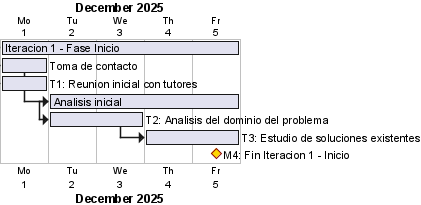
\includegraphics[width=0.98\linewidth]{gantt-inicio1.png}
    \caption{Diagrama de Gantt~--- Fase Inicio, Iteración 1}
    \label{fig:gantt_inicio1}
\end{figure}

\begin{figure}[H]
    \centering
    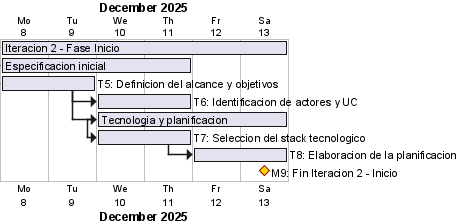
\includegraphics[width=0.98\linewidth]{gantt-inicio2.png}
    \caption{Diagrama de Gantt~--- Fase Inicio, Iteración 2}
    \label{fig:gantt_inicio2}
\end{figure}

\begin{figure}[H]
    \centering
    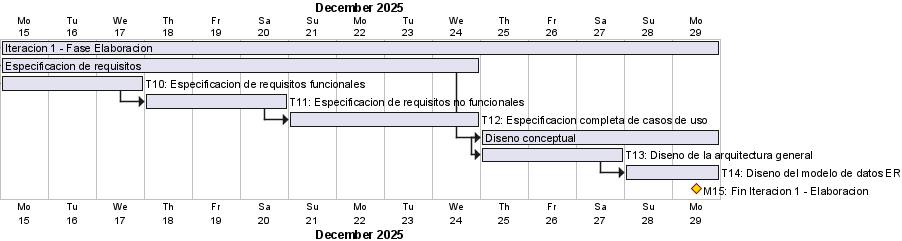
\includegraphics[width=0.98\linewidth]{gantt-elab1.png}
    \caption{Diagrama de Gantt~--- Fase Elaboración, Iteración 1}
    \label{fig:gantt_elab1}
\end{figure}

\begin{figure}[H]
    \centering
    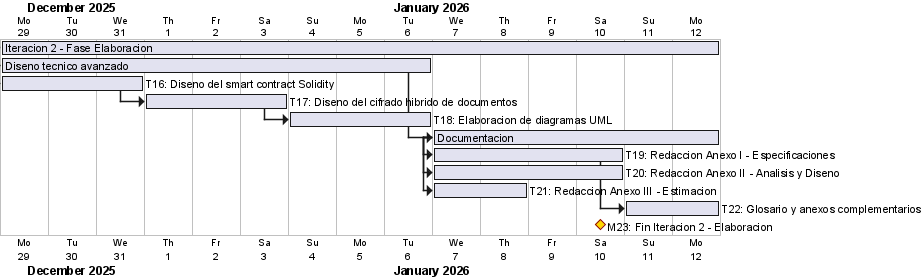
\includegraphics[width=0.98\linewidth]{gantt-elab2.png}
    \caption{Diagrama de Gantt~--- Fase Elaboración, Iteración 2}
    \label{fig:gantt_elab2}
\end{figure}

\begin{figure}[H]
    \centering
    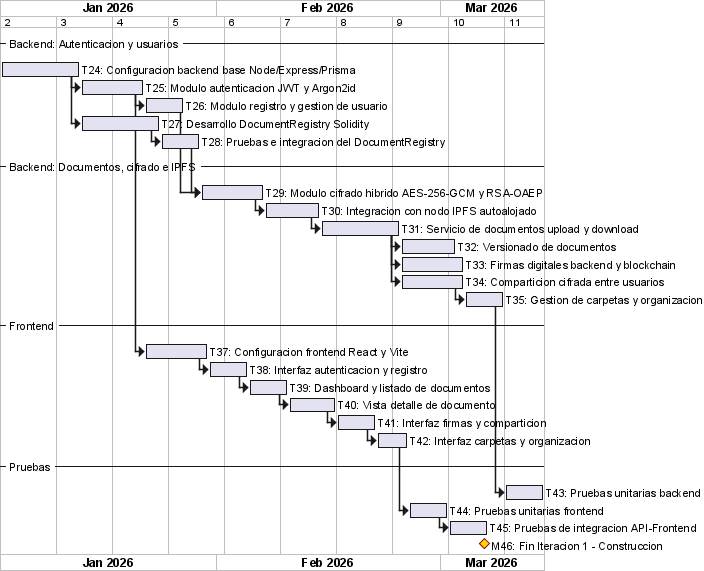
\includegraphics[width=0.98\linewidth]{gantt-const1.png}
    \caption{Diagrama de Gantt~--- Fase Construcción, Iteración 1}
    \label{fig:gantt_const1}
\end{figure}

\begin{figure}[H]
    \centering
    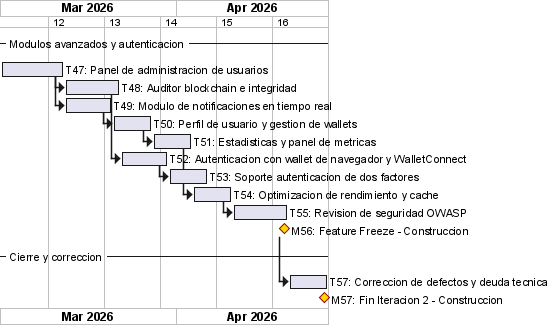
\includegraphics[width=0.98\linewidth]{gantt-const2.png}
    \caption{Diagrama de Gantt~--- Fase Construcción, Iteración 2}
    \label{fig:gantt_const2}
\end{figure}

\begin{figure}[H]
    \centering
    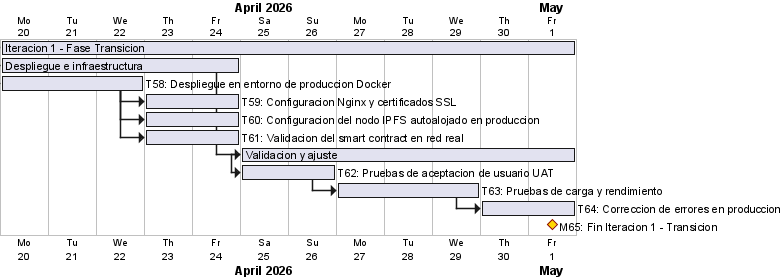
\includegraphics[width=0.98\linewidth]{gantt-trans1.png}
    \caption{Diagrama de Gantt~--- Fase Transición, Iteración 1}
    \label{fig:gantt_trans1}
\end{figure}

\begin{figure}[H]
    \centering
    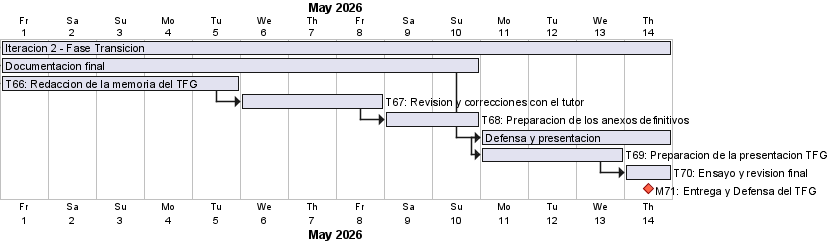
\includegraphics[width=0.98\linewidth]{gantt-trans2.png}
    \caption{Diagrama de Gantt~--- Fase Transición, Iteración 2}
    \label{fig:gantt_trans2}
\end{figure}

\section{Conclusiones}

Una vez definida la estimación del coste de desarrollo del proyecto DocumentChain y establecida la planificación temporal detallada mediante las distintas tablas de asignación de tiempos y el cronograma de iteraciones, se puede concluir que se trata de un proyecto de considerable complejidad tanto a nivel funcional como tecnológico. Esta complejidad no viene determinada únicamente por el número de casos de uso implementados (42 UC en 9 paquetes), sino también por la integración de cuatro subsistemas heterogéneos que requieren tecnologías de naturaleza muy distinta.

El proyecto DocumentChain combina un frontend React para la operación de usuario y la gestión local del material criptográfico, un backend Node.js con lógica de negocio compleja (cifrado AES-256-GCM, encapsulado RSA-OAEP de claves e integración blockchain), una capa de almacenamiento IPFS abstraída mediante un proveedor configurable y un smart contract Solidity que actúa como registro inmutable de la cadena de custodia documental. Cada uno de estos subsistemas ha requerido fases específicas de análisis, diseño, implementación y pruebas.

La estimación obtenida mediante la herramienta EZEstimate, con un total de \textbf{1.500 horas} de trabajo efectivo, ha resultado coherente con el esfuerzo real finalmente dedicado al desarrollo. Es importante destacar que esta estimación debe entenderse como una referencia orientativa para la planificación, ya que durante el desarrollo han surgido tareas adicionales no siempre reflejadas explícitamente en los casos de uso, tales como investigación tecnológica sobre blockchain, resolución de problemas de sincronización de eventos, ajustes de arquitectura de cifrado y pruebas continuas de seguridad.

Este análisis pone de manifiesto la importancia de definir con precisión los requisitos y objetivos durante las fases iniciales del proyecto (Inicio y Elaboración), ya que estas fases han servido como base para minimizar esfuerzos y garantizar la coherencia del sistema durante la fase de Construcción. La correcta estructuración de las iteraciones y la separación clara de responsabilidades entre los subsistemas han permitido abordar el desarrollo de forma progresiva y controlada.

\begin{table}[H]
\centering
\begin{tabular}{|p{4cm}|p{10cm}|}
\hline
\textbf{Fase (Iteración)} & \textbf{Descripción} \\
\hline
\textbf{Inicio} (Iteración 1) &
Primera toma de contacto con el proyecto DocumentChain. Se analizó el problema de la gestión documental segura y se estudiaron las soluciones existentes y sus limitaciones respecto a privacidad y trazabilidad blockchain. Se celebraron las primeras reuniones con los tutores para definir el alcance y los objetivos generales del trabajo. \\
\hline
\textbf{Inicio} (Iteración 2) &
Se definieron con mayor detalle los objetivos del sistema, los actores implicados y los primeros casos de uso. Se estableció la planificación inicial del proyecto y se seleccionaron las tecnologías principales (React, Node.js, PostgreSQL, Solidity, IPFS), justificando la elección de cada una. \\
\hline
\textbf{Elaboración} (Iteración 1) &
Se realizó el análisis detallado del sistema, definiendo los requisitos funcionales (IRQ) y no funcionales (NFR). Se diseñó la arquitectura general de cuatro capas identificando los subsistemas (frontend, backend, IPFS y blockchain) y sus relaciones. Se elaboró el diagrama Entidad-Relación de la base de datos. \\
\hline
\textbf{Elaboración} (Iteración 2) &
Se completaron los aspectos teóricos del proyecto, incluyendo el diseño del smart contract DocumentRegistry, el sistema de cifrado híbrido para documentos privados, los diagramas UML (clases, secuencia, componentes, despliegue) y la documentación técnica completa (Anexos I, II y III). \\
\hline
\textbf{Construcción} (Iteración 1) &
Primera iteración de implementación: subsistemas centrales del sistema. Se desarrolló el backend Node.js con autenticación JWT y soporte de wallets compatibles, el smart contract Solidity, la integración con la capa IPFS, el cifrado híbrido de documentos privados, los servicios de documentos/versiones/firmas/compartición/organización y el frontend React completo con sus páginas principales. \\
\hline
\textbf{Construcción} (Iteración 2) &
Segunda iteración de implementación: funcionalidades avanzadas. Se añadieron auditoría, estadísticas, panel de administración, notificaciones y email. Se realizaron las pruebas E2E con Playwright, la optimización del rendimiento, la validación de seguridad y la corrección de bugs. \\
\hline
\textbf{Transición} (Iteración 1) &
Se configuró y desplegó el sistema completo en un VPS con Docker Compose, incluyendo el backend, la base de datos PostgreSQL, la integración con el proveedor IPFS seleccionado y el smart contract en la red de pruebas Ethereum Sepolia. Se realizaron pruebas funcionales completas en el entorno de producción. \\
\hline
\textbf{Transición} (Iteración 2) &
Cierre del proyecto académico. Se redactó la memoria principal del TFG, se revisaron los anexos, se preparó la presentación de la defensa oral y se realizó la entrega oficial del proyecto a los tutores. \\
\hline
\end{tabular}
\caption{Descripción de las fases por iteraciones}
\end{table}

\section*{Bibliografía}
\addcontentsline{toc}{section}{Bibliografía}

\begin{enumerate}
    \item Karner, G. (1993). \textit{Metrics for Objectory} [Diploma thesis]. University of Linköping, Sweden.
    \item Schneider, G., \& Winters, J. (1998). \textit{Applying Use Cases: A Practical Guide}. Addison-Wesley.
    \item Cockburn, A. (2000). \textit{Writing Effective Use Cases}. Addison-Wesley Professional.
    \item Jacobson, I., Booch, G., \& Rumbaugh, J. (1999). \textit{The Unified Software Development Process}. Addison-Wesley.
    \item Sommerville, I. (2015). \textit{Software Engineering} (10.\textordfeminine\,ed.). Pearson.
    \item Ribu, K. (2001). \textit{Estimating Object-Oriented Software Projects with Use Cases} [Master's thesis]. University of Oslo.
\end{enumerate}

\end{document}
